
In this section, I will introduce core ideas behind dynamic compilation
of Rust lang. The section will present \textit{benefits of 
dynamic compilation} over the static one; talk about 
\textit{static borrow checker} and how it is integrated within the compilation
system; and discuss the \textit{modularity} achieved by separating concerns
into their own ``modules''.

Despite the aforementioned ideas, I should mention the idea of 
decreased compilation time. I only note that idea here due to
not having implemented it in the project, \textit{yet}. The virtual machine 
(i.e., interpreter and compiler, for now) implementation should
handle most of the language; its essential features such as closures,
lifetimes, templates, and so on. Because there is no support for more
advanced language constructs, there is no point in running
full-fledged benchmarks to compare the static and dynamic
compilers. Therefore, the focus of this paper is the challenge in separating
static (dataflow) analysis such as borrow checking from the core compilation
logic (i.e., code generation) so that the system can attempt to 
dynamically compile Rust.

\subsection{Benefits of Dynamic Compilation}

There are two ways to dynamically compile a language.
First, the naive way, would be to only use \textit{interpreter}. It takes
the source code and directly \textit{executes} it, without performing
any optimization transformations. As expected,
performance degrades rapidly; since source code on its own
may not be efficient without optimizations, executing it directly
will take much more time than to compile it \textit{ahead-of-time} (AOT) and
then run the executable.

On the other hand, just-in-time (JIT) compilation may combine the power of 
both interpreters and JIT compilers. Instead of directly executing code,
we could compile it to some intermediate representation (IR), run optimization
on that IR, and then compile and execute it.

There are several benefits from JIT compilation\textcolor{red}{cite presentationhttp://www.cs.columbia.edu/~aho/cs6998/Lectures/14-09-22\_Croce\_JIT.pdf}. First, JIT compiler uses
only a fraction of memory that AOT compiler would because we do not have
to compile entire program at once; we simply compile whatever is necessary 
``now'' (i.e., compiling a method being currently called). After obtaining
machine code, we cache the function (and possibly its result for some
state and arguments) so that we do not have to re-compile it again. Hence,
we only focus on the necessary and frequently-called functions.

Unlike interpreters, JIT compilers can also gather statistics about
called methods at runtime. Knowing which methods are the \textit{hotspots} (places
where a program spends most of the time executing) and/or are frequently called,
JIT compiler may aim on optimizing these more aggressively. In addition,
JIT compilers may leverage target-specific optimizations that interpreters 
ignore completely. Therefore, JIT compilation provides a better (``smarter'')
way to turn high-level source code into native machine code.

% Interpretation vs JIT. Less memory demand, since we only compile
% executed methods.
% JIT is better than interpreter - we can collect stats, leverage
% target-specific optimizations,
%

\subsection{Static borrow checker}
{%
\floatstyle{plain}
\restylefloat{figure}
\begin{figure}
    %\begin{center}
        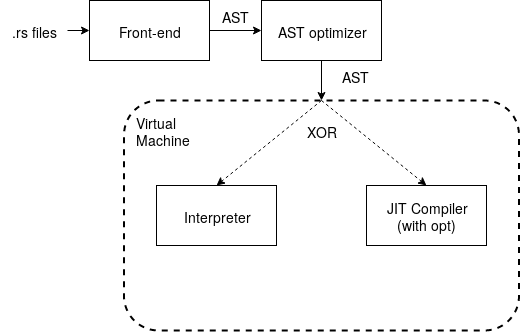
\includegraphics[width=0.5\textwidth]{architecture.png}
    %\end{center}
    \caption{High-level architecture of the system.}
    \label{arch1}
\end{figure}
}
\begin{figure*}[ht]
    \begin{center}
        \lstinputlisting{ast.cpp}
    \end{center}
    \caption{AST.hpp maps each rule to its own class.}
    \label{cpp1}
\end{figure*}

\texttt{rustc} generates and uses (sequentially) three levels of IR. While
performing static program analysis such as liveness or pointer analysis, Rust
compiler refers to (i.e., copies and/or transforms) the mid-level IR (MIR),
which is obtained from the high-level IR. The MIR is a \textcolor{red}{ cite
https://rust-lang.github.io/rustc-guide/mir/index.html}  control-flow
graph-based IR which provides explicit type information. Providing a program's
explicit execution flow, the MIR makes it possible to perform the
\textit{flow-sensitive} analysis such as borrow checking.

It is hardly possible to do analysis on the original source code. As an
interpreter directly executes the code, it cannot perform any of these checks.
Since I only implemented dynamic compilation for a subset of the language, it
can handle borrow checking analysis \textit{only}. However, as our project
starts to support more of the language, interpreter will not be able to perform
such checks \textit{quick enough} (or, at least, as quick as the original
static compiler).  We could handle that case by taking an inspiration from the
Java world, namely the HotSpot JVM \textcolor{red}{cite jvm
https://www.usenix.org/legacy/publications/library/proceedings/jvm01
/full\_papers/russell/russell\_html/index.html}. At a high level, JVM is a
system with two compilers: an AOT compiler, which reads source code, performs
(if any useful) optimization transformations, and outputs the corresponding
bytecode; and a JIT compiler, which then takes the bytecode, optimizes it,
compiles and executes it. In a similar fashion, I present a system with two
separate compilers (see \hyperref[arch1]{Figure 3}): the front-end compilers
that outputs tree-based (abstract syntax tree, or AST) representation,
optimizes it statically, and outputs a better AST; and the virtual machine that
takes the AST and either interprets it, or JIT-compiles it into a machine code
(which is then executed).

Due to the separation of concerns (i.e., \textit{static} front-end 
and \textit{dynamic} interpreter and JIT compiler), the system attains
high modularity and less coupling. The modular design
allows for better unit and integration testing, as well as
easier debugging via isolation of the components.

